\chapter{Mediator模式}
\section{Mediator模式的概念}
\subsection{定义}
中介者(Mediator)模式的定义:定义一个中介对象来封装一系列对象之间的交互,使原有对象之间的耦合松散,且可以独立地改变它们之间的交互。中介者模式又叫调停模式,它是迪米特法则的典型应用。
\subsection{优点}
\begin{enumerate}
	\item 降低了对象之间的耦合性,使得对象易于独立地被复用;
	\item 将对象间的一对多关联转变为一对一的关联,提高系统的灵活性,使得系统易于维护和扩展。
\end{enumerate}
\subsection{缺点}
\begin{enumerate}
	\item 当同事类太多时,中介者的职责将很大,它会变得复杂而庞大,以至于系统难以维护。
\end{enumerate}
\subsection{应用场景}
\begin{enumerate}
	\item 当对象之间存在复杂的网状结构关系而导致依赖关系混乱且难以复用时。
	\item 当想创建一个运行于多个类之间的对象,又不想生成新的子类时。
\end{enumerate}
\subsection{中介者模式的角色}
\begin{enumerate}
	\item Mediator仲裁者/中介者:它是中介者的接口,提供了同事对象注册与转发同事对象信息的抽象方法。
	\item ConcreteMediator具体中介者:实现中介者接口,定义一个 List 来管理同事对象,协调各个同事角色之间的交互关系,因此它依赖于同事角色。
	\item Colleague同事:定义同事类的接口,保存中介者对象,提供同事对象交互的抽象方法,实现所有相互影响的同事类的公共功能。
	\item ConcreteColleague具体同事:是抽象同事类的实现者,当需要与其他同事对象交互时,由中介者对象负责后续的交互。
\end{enumerate}
\section{中介者模式实现——例一}
\begin{figure}[!h]
	\centering
	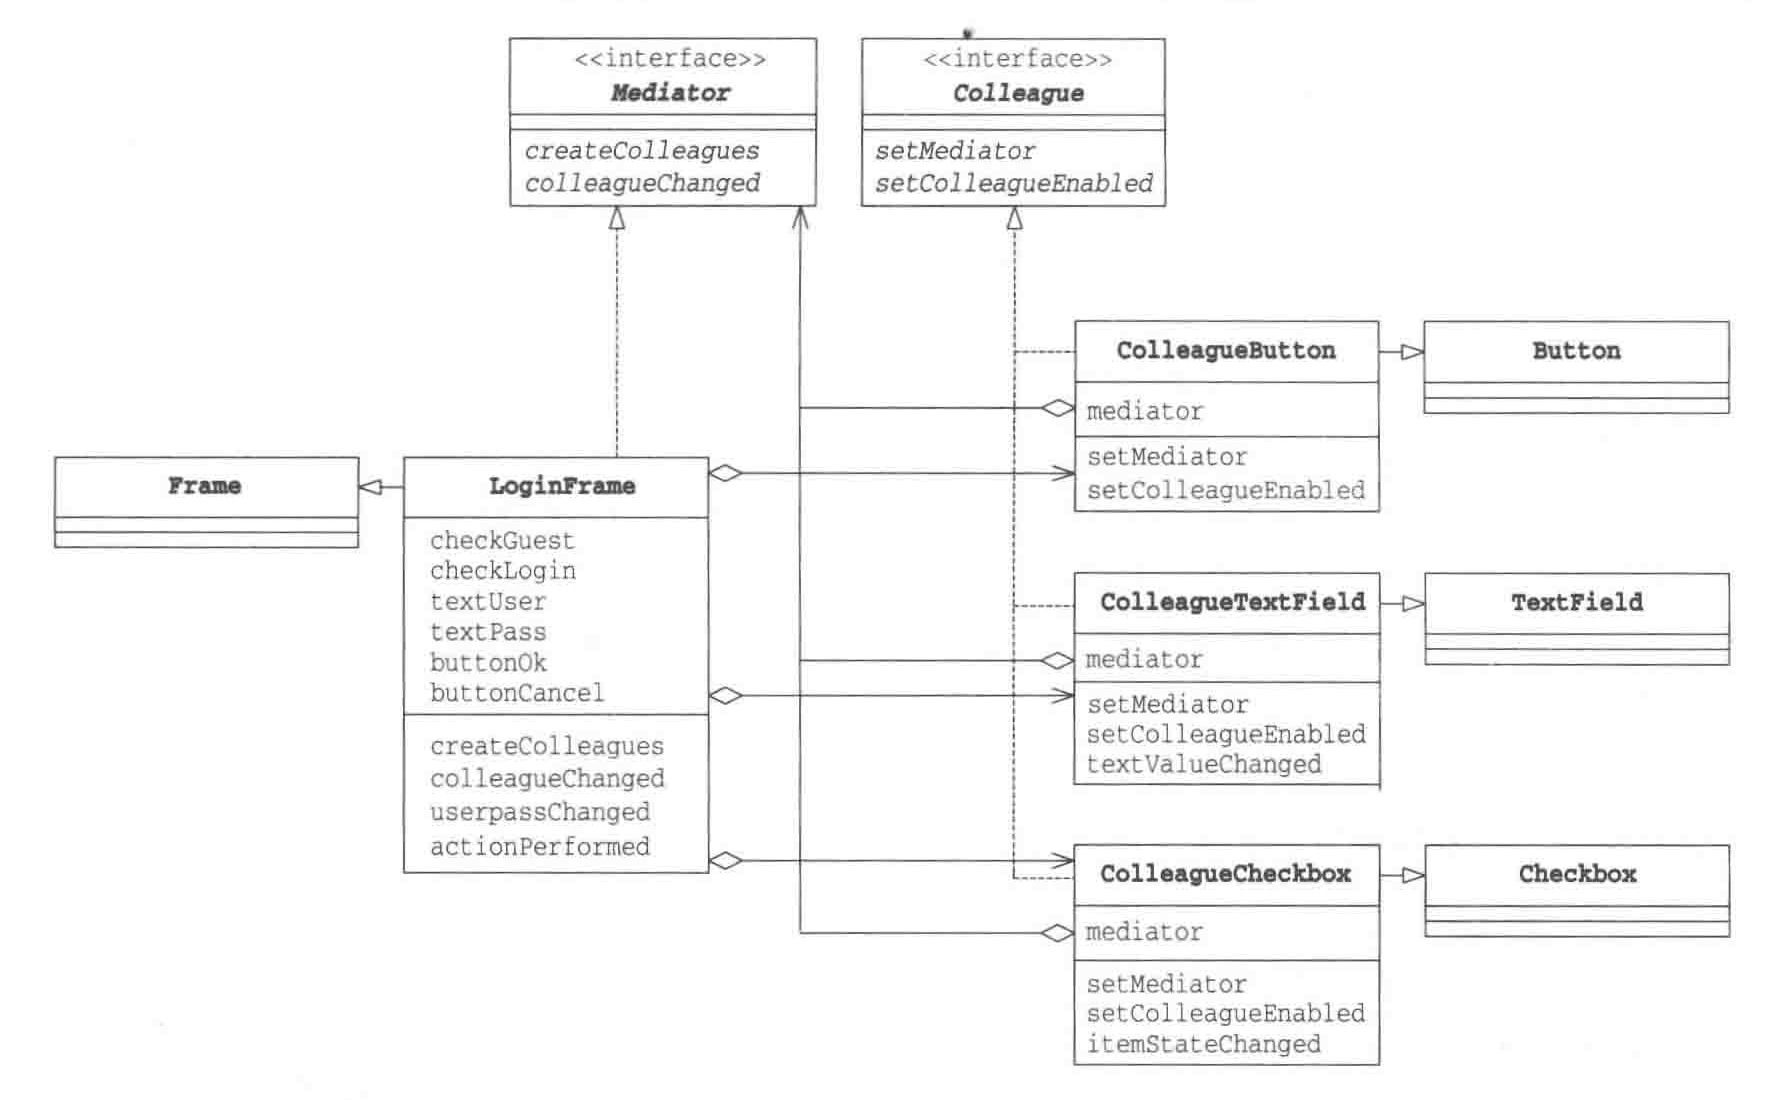
\includegraphics[width=\textwidth]{image/16-1}
	\caption{中介者模式结构图}
\end{figure}
\begin{figure}[!h]
	\centering
	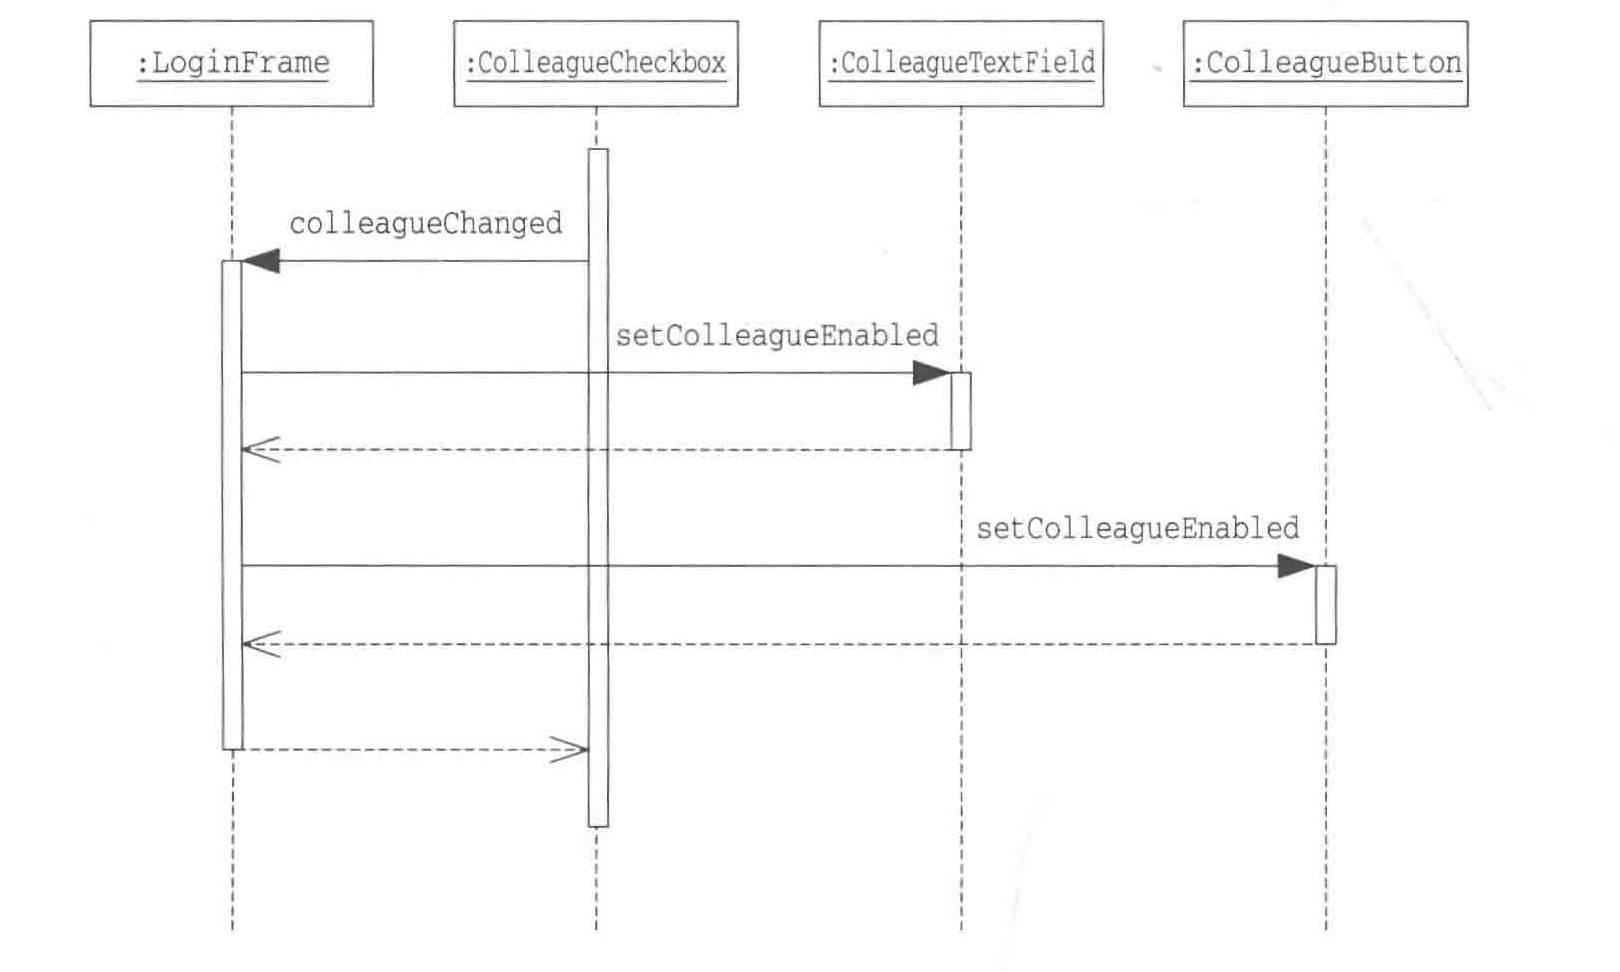
\includegraphics[width=\textwidth]{image/16-2}
	\caption{中介者模式顺序图}
\end{figure}
\begin{lstlisting}
public interface Colleague {
	//让组员知道仲裁者
	void SetMediator(Mediator mediator);
	//告知组员仲裁者下达的命令,在这个例子中就是启用或不启用
	void setColleagueEnabled(boolean enabled);
}
public interface Mediator {
	// 生成组员API
	void createColleague();
	//被各个 Colleague 使用,向仲裁者报告
	void colleagueChanged();
}
\end{lstlisting}
\begin{lstlisting}
//登录框的按钮
public class ColleagueButton extends Button implements Colleague {
	private Mediator mediator;
	public ColleagueButton(String label) throws HeadlessException {
		super(label);
	}
	public void SetMediator(Mediator mediator) {
		this.mediator = mediator;
	}
	public void setColleagueEnabled(boolean enabled) {
		setEnabled(enabled);
	}
}
\end{lstlisting}
\begin{lstlisting}
public class ColleagueCheckbox extends Checkbox implements ItemListener, Colleague {
	private Mediator mediator;
	public ColleagueCheckbox(String label, CheckboxGroup group, boolean state) throws HeadlessException {
		super(label, group, state);
	}
	public void SetMediator(Mediator mediator) {
		this.mediator = mediator;
	}
	public void setColleagueEnabled(boolean enabled) {
		setEnabled(enabled);
	}
	// 状态改变时调用
	public void itemStateChanged(ItemEvent e) {
		mediator.colleagueChanged();
	}
}
\end{lstlisting}
\begin{lstlisting}
// 登录窗口的文本框
public class ColleagueTextField extends TextField implements TextListener, Colleague {
	private Mediator mediator;
	public ColleagueTextField(String text, int columns) throws HeadlessException {
		super(text, columns);
	}
	public void SetMediator(Mediator mediator) {
		this.mediator = mediator;
	}
	public void setColleagueEnabled(boolean enabled) {
		setEnabled(enabled);
		setBackground(enabled ? Color.WHITE : Color.lightGray);
	}
	// 当文字发生变化是通知 Meditor
	public void textValueChanged(TextEvent e) {
		mediator.colleagueChanged();
	}
}
\end{lstlisting}
\begin{lstlisting}
// 作为仲裁者
public class LoginFrame extends Frame implements ActionListener, Mediator {
	private ColleagueCheckbox checkGuest;
	private ColleagueCheckbox checkLogin;
	private ColleagueTextField textUser;
	private ColleagueTextField textPass;
	private ColleagueButton buttonOk;
	private ColleagueButton buttonCancel;
	public LoginFrame(String title) throws HeadlessException {
		super(title);
		// 设置颜色
		setBackground(Color.lightGray);
		// 设置布局
		setLayout(new GridLayout(4, 2));
		// 创建组件
		createColleague();
		add(checkGuest);
		add(checkLogin);
		add(new Label("Username: "));
		add(textUser);
		add(new Label("Password: "));
		add(textPass);
		add(buttonOk);
		add(buttonCancel);
		// 设置初始状态
		colleagueChanged();
		pack();
		show();
	}
	public void createColleague() {
		CheckboxGroup group = new CheckboxGroup();
		checkGuest = new ColleagueCheckbox("Guest", group, true);
		checkLogin = new ColleagueCheckbox("Login", group, false);
		textUser = new ColleagueTextField("", 10);
		textPass = new ColleagueTextField("", 10);
		textPass.setEchoChar('*');
		buttonOk = new ColleagueButton("OK");
		buttonCancel = new ColleagueButton("Cancel");
		checkGuest.SetMediator(this);
		checkLogin.SetMediator(this);
		textUser.SetMediator(this);
		textPass.SetMediator(this);
		buttonCancel.SetMediator(this);
		buttonOk.SetMediator(this);
		checkGuest.addItemListener(checkGuest);
		checkLogin.addItemListener(checkLogin);
		textUser.addTextListener(textUser);
		textPass.addTextListener(textPass);
		buttonOk.addActionListener(this);
		buttonCancel.addActionListener(this);
	}
	public void colleagueChanged() {
		if (checkGuest.getState()) {    //游客模式
			textUser.setColleagueEnabled(false);
			textPass.setColleagueEnabled(false);
			buttonOk.setColleagueEnabled(true);
		} else {                        //用户模式
			textUser.setColleagueEnabled(true);
			userpassChanged();
		}
	}
	
	private void userpassChanged() {
		if (textUser.getText().length() > 0) {
			textPass.setColleagueEnabled(true);
			if (textPass.getText().length() > 0) {
				buttonOk.setColleagueEnabled(true);
			} else {
				buttonOk.setColleagueEnabled(false);
			}
		} else {
			textPass.setColleagueEnabled(false);
			buttonOk.setColleagueEnabled(false);
		}
	}
	public void actionPerformed(ActionEvent e) {
		System.out.println(e.toString());
		System.exit(0);
	}
}
\end{lstlisting}
\begin{lstlisting}
public class Main {
	public static void main(String[] args) {
		new LoginFrame("Mediator Sample");
	}
}
\end{lstlisting}
\section{中介者模式实现——例二}
\begin{figure}[!h]
	\centering
	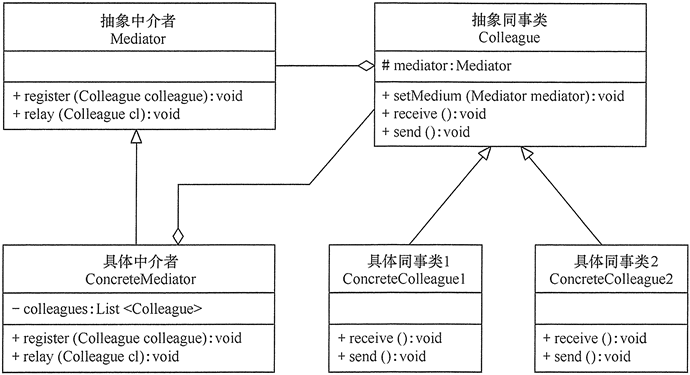
\includegraphics[width=0.8\textwidth]{image/16-3}
	\caption{中介者模式结构图}
\end{figure}
\begin{lstlisting}
//抽象中介者
abstract class Mediator {
	public abstract void register(Colleague colleague);
	public abstract void relay(Colleague cl); //转发
}

//具体中介者
class ConcreteMediator extends Mediator {
	private List<Colleague> colleagues = new ArrayList<Colleague>();
	public void register(Colleague colleague) {
		if (!colleagues.contains(colleague)) {
			colleagues.add(colleague);
			colleague.setMedium(this);
		}
	}
	public void relay(Colleague cl) {
		for (Colleague ob : colleagues) {
			if (!ob.equals(cl)) {
				((Colleague) ob).receive();
			}
		}
	}
}
\end{lstlisting}
\begin{lstlisting}
//抽象同事类
abstract class Colleague {
	protected Mediator mediator;
	public void setMedium(Mediator mediator) {
		this.mediator = mediator;
	}
	public abstract void receive();
	public abstract void send();
}

//具体同事类
class ConcreteColleague1 extends Colleague {
	public void receive() {
		System.out.println("具体同事类1收到请求。");
	}
	public void send() {
		System.out.println("具体同事类1发出请求。");
		mediator.relay(this); //请中介者转发
	}
}

//具体同事类
class ConcreteColleague2 extends Colleague {
	public void receive() {
		System.out.println("具体同事类2收到请求。");
	}
	public void send() {
		System.out.println("具体同事类2发出请求。");
		mediator.relay(this); //请中介者转发
	}
}
\end{lstlisting}
\begin{lstlisting}
public class MediatorPattern {
	public static void main(String[] args) {
		Mediator md = new ConcreteMediator();
		Colleague c1, c2;
		c1 = new ConcreteColleague1();
		c2 = new ConcreteColleague2();
		md.register(c1);
		md.register(c2);
		c1.send();
		System.out.println("-------------");
		c2.send();
	}
}
\end{lstlisting}
\begin{lstlisting}
//output
具体同事类1发出请求。
具体同事类2收到请求。
-------------
具体同事类2发出请求。
具体同事类1收到请求。
\end{lstlisting}
\section{模式扩展}
在实际开发中,通常采用以下两种方法来简化中介者模式,使开发变得更简单。
\begin{enumerate}
	\item 不定义中介者接口,把具体中介者对象实现成为单例。
	\item 同事对象不持有中介者,而是在需要的时f矣直接获取中介者对象并调用。
\end{enumerate}
\begin{figure}[!h]
	\centering
	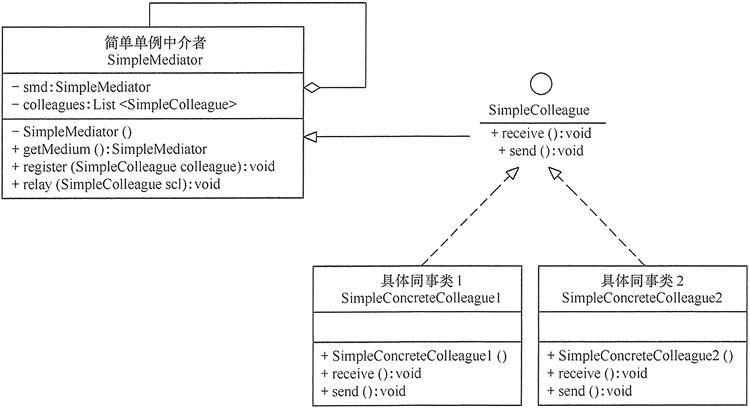
\includegraphics[width=0.8\textwidth]{image/16-4}
	\caption{简化中介者模式的结构图}
\end{figure}
\begin{lstlisting}
//简单单例中介者
class SimpleMediator {
	private static SimpleMediator smd = new SimpleMediator();
	private List<SimpleColleague> colleagues = new ArrayList<SimpleColleague>();
	private SimpleMediator() {}
	public static SimpleMediator getMedium() {
		return (smd);
	}
	public void register(SimpleColleague colleague) {
		if (!colleagues.contains(colleague)) {
			colleagues.add(colleague);
		}
	}
	public void relay(SimpleColleague scl) {
		for (SimpleColleague ob : colleagues) {
			if (!ob.equals(scl)) {
				((SimpleColleague) ob).receive();
			}
		}
	}
}
\end{lstlisting}
\begin{lstlisting}
//抽象同事类
interface SimpleColleague {
	void receive();
	void send();
}
//具体同事类
class SimpleConcreteColleague1 implements SimpleColleague {
	SimpleConcreteColleague1() {
		SimpleMediator smd = SimpleMediator.getMedium();
		smd.register(this);
	}
	public void receive() {
		System.out.println("具体同事类1:收到请求。");
	}
	public void send() {
		SimpleMediator smd = SimpleMediator.getMedium();
		System.out.println("具体同事类1:发出请求...");
		smd.relay(this); //请中介者转发
	}
}

//具体同事类
class SimpleConcreteColleague2 implements SimpleColleague {
	SimpleConcreteColleague2() {
		SimpleMediator smd = SimpleMediator.getMedium();
		smd.register(this);
	}
	public void receive() {
		System.out.println("具体同事类2:收到请求。");
	}
	public void send() {
		SimpleMediator smd = SimpleMediator.getMedium();
		System.out.println("具体同事类2:发出请求...");
		smd.relay(this); //请中介者转发
	}
}
\end{lstlisting}
\begin{lstlisting}
public class SimpleMediatorPattern {
	public static void main(String[] args) {
		SimpleColleague c1, c2;
		c1 = new SimpleConcreteColleague1();
		c2 = new SimpleConcreteColleague2();
		c1.send();
		System.out.println("-----------------");
		c2.send();
	}
}
\end{lstlisting}
\section{扩展思路}
\begin{enumerate}
	\item 当发生分散灾难时,即各个中介者和同事交互的colleagueChanged发生发生bug时,其他地方并没有控制控件的启用/禁用状态的逻辑处理,可以迅速排除bug。避免处理过于集中,分而治之。
	\item 可以减弱通信线路的增加。
	\item ConcreteColleague可以复用,但ConcreteMediator很难复用。
\end{enumerate}
\section{相关设计模式}
\begin{enumerate}
	\item Facade中,Facade角色单方面地使用其他角色来对外提供高层接口(单向的);Mediator中,Mediator角色与Colleague进行交互(双向)。
	\item 可以使用Observer模式实现Mediator角色和Colleague角色之间的通信。
\end{enumerate}